\section{Repository architecture}

The general architecture of our code repository is explained in this tree :\\

\begin{figure}[!h] 
\begin{center}
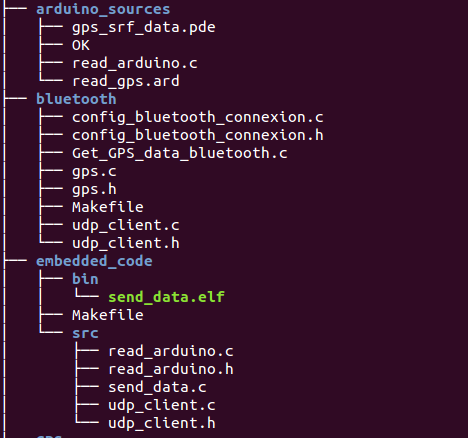
\includegraphics[width=10cm]{imgs/c1.png}
\caption{1st part of the repository} 
\label{img1} 
\end{center}
\end{figure} 

In arduino\_sources folder, all the code related to the arduino board can be found.
The software used to program the arduino is expecting .pde or .ard files.\\

In the following parts, we will provide more details for each files.\\

The bluetooth folder contains C sources et headers used on the target to catch informations sent by the smartphone.\\

The embedded code section includes all the programs we created to run on the UAV embedded linux.\\

\newpage

\begin{figure}[!h] 
\begin{center}
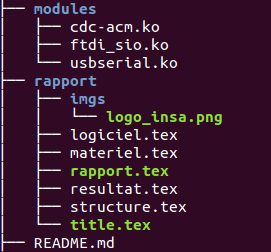
\includegraphics[width=7cm]{imgs/c2.png}
\caption{2nd part of the repository} 
\label{img1} 
\end{center}
\end{figure} 

All the compiled modules we added on the embedded linux can be found in the module folder.\\

The ``rapport'' directory contains the sources of the documentation you are reading !\\

Finally, the most important folder is the one named sdk\_apps. It contains one application named auto\_flight. Like most of the c projects, you can find a Makefile, a bin/ and a src/ folder. The Makefile is configurated to create the application binary and to move it to the bin/ folder. You can find additionnal informations about the Makefile in the appedices.\\

About the src/ folder :\\

The most important C file is named ardrone\_testing\_tool.c. This file is making the link between our application and the ARdrone library. Moreover, it is launching and joining all our threads.\\

The Auto/ folder contains code related to the auto\_control thread.\\

The Avoidance/ folder contains code related to the avoidance thread.\\

The Comm/ folder contains code related to the receive\_gps thread.\\

The Comm\_target/ folder contains code related to the gps\_target thread.\\

The Control/ folder contains an small library we wrote to handle UAV travelling.\\

The GPS/ folder contains algorithms used to manipulate GPS strings and make distance and angle calculation.

The Navdata/ folder contains the fonctions used to read and store navdata sent by the UAV.\\

The STMachine/ folder contains the fonctions generated by SCADE KCG compiler.\\

The Target/ folder contains code related to the target thread.\\

\begin{figure}[!h] 
\begin{center}
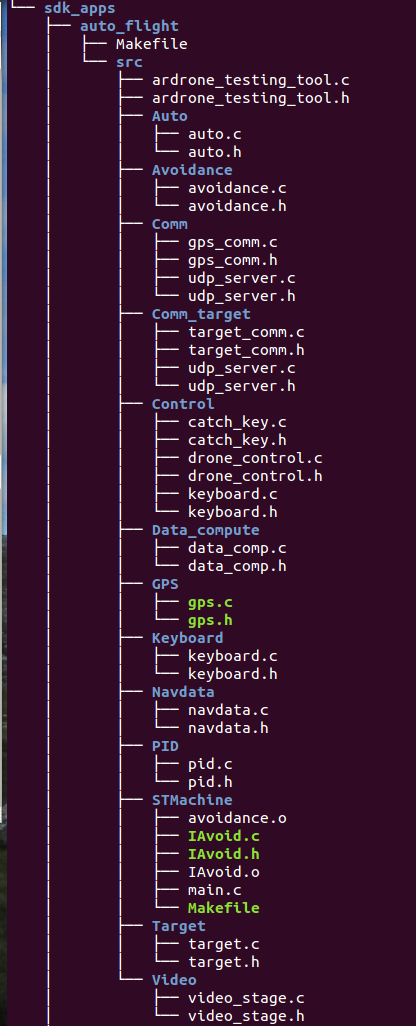
\includegraphics[width=8cm]{imgs/c3.png}
\caption{3rd part of the repository} 
\label{img1} 
\end{center}
\end{figure} 

\newpage{}

\begin{tabular}{|l|l|l|}
    \hline
    Thread name & Period & Description \tabularnewline
    \hline
    ardrone\_control & 2 & Library related thread \tabularnewline
    \hline
    navdata\_update & 20 & Library related thread \tabularnewline
    \hline
    auto\_control & 20 & Thread allowing manual command of the UAV \tabularnewline
    \hline
    receive\_gps & 50 & Thread used to received gps coordinated sent by the UAV  \tabularnewline
    \hline
    avoidance & 60    & Thread used to perform autonomous obstacle avoidance   \tabularnewline
    \hline
    gps\_target & 50 & Thread used to received gps coordinated sent by the target  \tabularnewline
    \hline
    gps\_target & 50 & Thread used to perform autonomous convergence to the target  \tabularnewline
    \hline

 \end{tabular}

This table summarizes all the thread launched in our application. In the following sections, we will detail the operations of each threads.

\section{The auto thread}

The auto thread is mainly based on the movement API we developped with the Brown team.\\

\subsection{Movement API}

This API is an overlay of the Parrot API, it allows more intuitive UAV control. It also provide movement quatification, which means you can quantify an order by speed, distance or duration. For example, you can emit orders like ``go forward on 300 cm''.

\subsubsection{Les mouvements élémentaires}

Les commandes de déplacement sont définis dans le fichier Control/drone\_control.c, elles ont toutes le même format :

The travelling commands are all defined in the file Control/drone\_control.c, they have the same format :\\

\begin{lstlisting}
C_RESULT ordre (void *arg)
\end{lstlisting}

The list of available travellings :\\

\begin{itemize}

\item turn\_left 
\item turn\_right
\item forward    
\item backward   
\item up         
\item down       
\item right      
\item left       
\item stop       

\end{itemize}

\subsection{Send an order}

The above order can be passed to both functions depending on whether you want to make a move that will be termed ``elementary'', or a longer trip by specifying the distance.

\subsubsection{Elementary move}

An elementary movement allows for a sudden displacement of around 10 cm. You must use the following function:

\begin{lstlisting}
C_RESULT small_move(ORDER* order)
\end{lstlisting}

Sample code :\\

\begin{lstlisting}
small_move(turn_right);
\end{lstlisting}

\subsubsection{Long move}

All orders to send move commands accept an argument of type void *. This argument must be cast to void * but available commands manage only the type arguments mov\_t which includes different arguments :\\

\begin{lstlisting}
typedef struct mov_t{
  int32_t power;     //engine power between 0 and 100 
  int32_t distance;  //distance in cm
  int32_t time;      //time in usec
}mov;
\end{lstlisting}

Before sending orders, it's important to fill correctly this structure. Unused fields must be initialized to -1. To send an order, this function must be used :\\

\begin{lstlisting}
C_RESULT send_order(ORDER* order, void *arg)
\end{lstlisting}

Sample code :\\

\begin{lstlisting}
/* 30% on 70 cm*/
mov mv = {30, 70, -1};
send_order(backward, &mv);
\end{lstlisting}

\subsection{Using of this API}

In the auto thread, we need to control the UAV with the keyboard of the station. This automatic control is really useful in case of problems occuring during the automatic control.\\

Basically, we are just running a scanf in an infinite loop. Depeding on the key pressed, we just have to call the wright function of the API.\\

\begin{lstlisting}
  while (1) {
    usleep(100000);
    scanf("%c", &c);
    printf("%c\n",c);
    switch(c){
    case 'f':
      small_move(forward);
      break;
    case 'b':
      small_move(backward);
      break;
    case 'u':
      small_move(up);
      break;
    case 'd':
      small_move(down);
      break;
    case 'o':
      //small_move(left);
      printf("Batt :%d\n",sauv_ndata.bat_level_current);
      break;
\end{lstlisting}

Very helpful functionalities are battery control, by pressing the ``o'' key, and recover from emergency m
ode by pressing ``x''. All the other command are pretty basic (``land'', ``go up'', ``go down'').\\

\subsection{Storing navdatas}

We also use this thread to store the navdata received. To achieve this goal, it is necessary to declare three functions, defined in the ARDrone library :\\

\begin{lstlisting}
/* Initialization local variables before event loop  */
inline C_RESULT auto_navdata_client_init( void* data )

/* Receving navdata during the event loop */
inline C_RESULT auto_navdata_client_process( const navdata_unpacked_t* const navdata )

/* Relinquish the local resources after the event loop exit */
inline C_RESULT auto_navdata_client_release( void )
\end{lstlisting}

We just keep the informations we have to use later, like battery level, control state, altitude or psi angle.

\begin{lstlisting}
  sauv_ndata.psi_current = nd->psi / 1000;
  sauv_ndata.bat_level_current = nd->vbat_flying_percentage;
  sauv_ndata.ctrl_state_current = nd->ctrl_state;
  sauv_ndata.tag_detected = nv->nb_detected;
  sauv_ndata.tag_tab = nv->camera_source;
  sauv_ndata.alt = nd->altitude / 1000.0;
\end{lstlisting}

We store all these informations in a global structure that will be accessed by the other threads.

\section{The avoidance thread}

This thread is mainly based on SCADE generated code. The statechart modeling the avoidance is printed below :\\

\begin{figure}[!h] 
\begin{center}

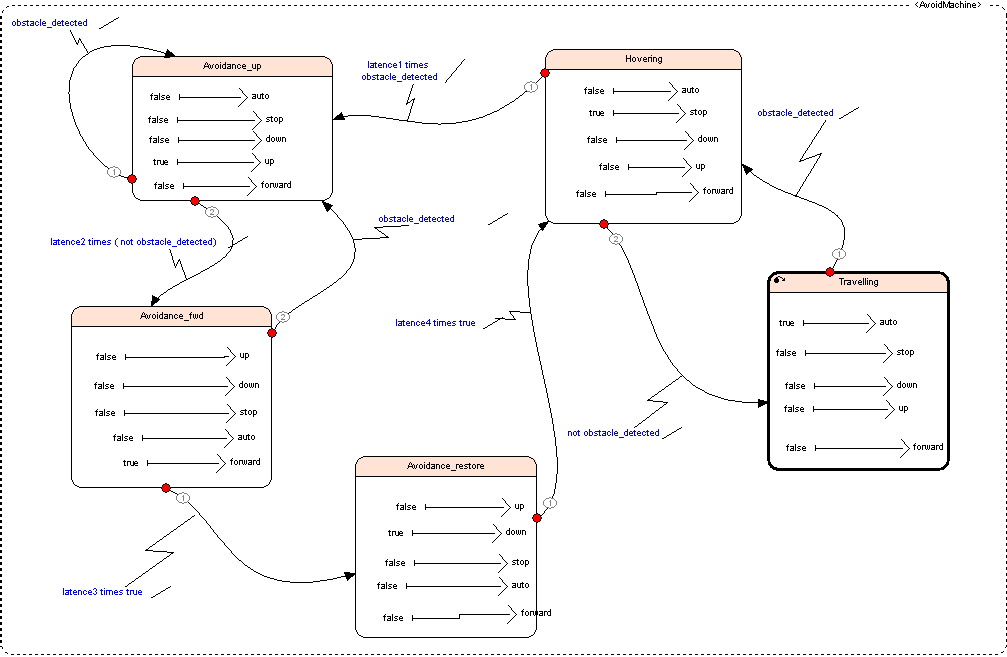
\includegraphics[width=19cm]{imgs/scade.png}
\caption{SCADE statechart} 
\label{img1} 
\end{center}
\end{figure} 

Then, the KCG compiler gave us some independent code, that we included in our project.

\begin{lstlisting}
switch (AvoidMachine_state_sel) {
    case SSM_st_Travelling_AvoidMachine :
      outC->AvoidMachine_reset_act = inC->obstacle_detected;
      break;
    case SSM_st_Hovering_AvoidMachine :
      if (br_1_guard_AvoidMachine_Hovering) {
        outC->AvoidMachine_reset_act = 1;
      }
      else {
        outC->AvoidMachine_reset_act = br_2_guard_AvoidMachine_Hovering;
      }
      outC->init = 0;
      break;
    case SSM_st_Avoidance_up_AvoidMachine :
      if (inC->obstacle_detected) {
        outC->AvoidMachine_reset_act = 1;
      }
      else {
        outC->AvoidMachine_reset_act = br_2_guard_AvoidMachine_Avoidance_up;
      }
      outC->init2 = 0;
      break;
\end{lstlisting}

The top-level function is defined in the file IAvoid.h.

\begin{lstlisting}
extern void IAvoid(inC_IAvoid *inC, outC_IAvoid *outC);
\end{lstlisting}

The inputs of this statechart are a boolean named ``obstacle\_detected'' (its value is 1 if there is an obstacle and 0 otherwise) and 4 integers describing latencies between transitions.\\

The outputs are 5 booleans : 4 orders (up, down, stop, forward) and a neutral order (if there is nothing to do).\\

Each call to the function represent a cycle. We have planned to execute a cycle each 10ms. The following code is illustrating the use of the auto-generated function :\\

\begin{lstlisting}
DEFINE_THREAD_ROUTINE(avoidance, data) {
  
  comm_datas datas;
  double dangerThreshold=100;
  int detection;
  double average_left;
  int ret;

  init_array_obstacle_pos2();

  IAvoid_reset(&output);
  input.obstacle_detected = 0;
  input.latence1 = 100;
  input.latence2 = 100;
  input.latence3 = 300;
  input.latence4 = 100;

 while (1) {
   usleep(10);
   if (auto_ready) {
     //get srf datas
     datas = get_comm_datas();

     ret = average_obstacle_pos2(&datas.srfr, &average_left);
     printf("Moyenne capteur(%d) : %f\n", ret, average_left);

     //check threshold
     if (average_left < dangerThreshold) {
       detection = 1;
     } else {
       detection = 0;
     } 
   
     input.obstacle_detected = detection;     
     IAvoid(&input,&output);
     command(output);
     usleep(10000);    
   }
 }
 
  return (THREAD_RET) 0;
}
\end{lstlisting}

And the command function is :\\

\begin{lstlisting}
void command(outC_IAvoid comm) {
  mov speed;

  if (comm.up) {
    speed.power = 8;
    send_fast_order(up,(void *)&speed);
  } else if (comm.down) {
    speed.power = 3;
    send_fast_order(down,(void *)&speed);
  } else if (comm.stop) {
    send_fast_order(stop,NULL);
  } else if (comm.auto1) {
    speed.power = 1;
    printf("avance\n");
    send_fast_order(forward,(void *)&speed);
  } else if (comm.forward) {
    speed.power = 1;
    printf("avance\n");
    send_fast_order(forward,(void *)&speed);
  }

}
\end{lstlisting}

\section{The receive\_gps \& gps\_target threads}

\section{The target thread}



